\section{Hauptteil}
\label{section:main}

Im Hauptteil dieser Arbeit wird die \glqq Carsharing Applikation\grqq anhand der im Theorieteil beschriebenen Entwurfsschritte: 1. Anforderungsanalyse, 2. ERM, und 3. Abbildung auf Relationenmodell entworfen. Anschließend wird die Datenbank in Racket übertragen und beispielhaft gezeigt, wie mit der Datenbanksprache SQL einzelne Datensätze erstellt und abgerufen werden können.

\subsection{Datenbankmodell einer \glqq Carsharing Applikation\grqq}

\paragraph{Schritt 1: Anforderungsanalyse}
In \autoref{fig:Anforderungsanalyse_Main} ist eine ausführliche Anforderungsanalyse der \glqq Carsharing Applikation\grqq dargestellt. Aus diesen Anforderungen können nun die Entitäten (Klassen), ihre Attribute und die Beziehungen abgeleitet und in ein ERM übertragen werden.

\begin{figure}[htb]
	\centering
	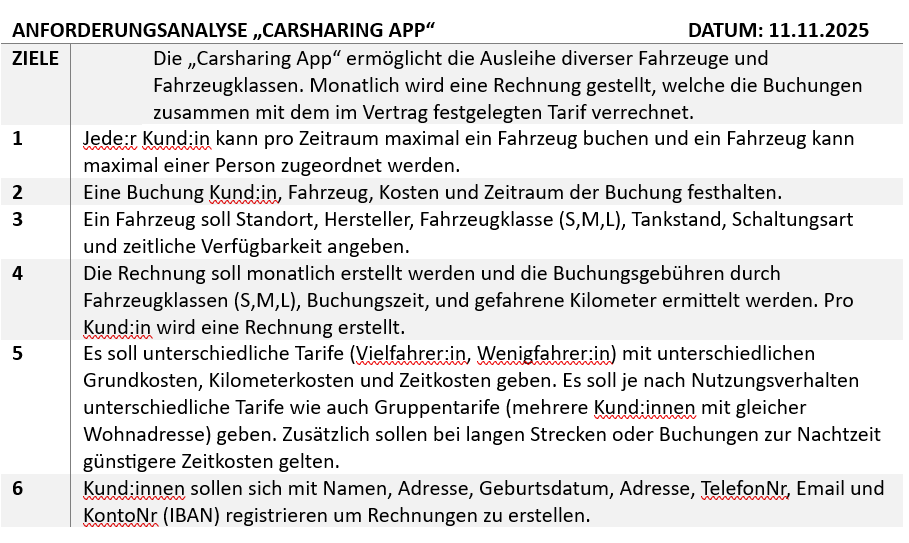
\includegraphics[width=\linewidth]{./pictures/Anforderungsliste_Main}
	\caption{Anforderungsanalyse für die \glqq Carsharing Applikation\grqq.}
	\label{fig:Anforderungsanalyse_Main}
\end{figure}

\paragraph{Schritt 2: Abbildung in ein ERM}
Für das ERM werden die relevanten Entitäten und Beziehungstypen aus dem Anforderungskatalog abgeleitet. Auf Basis des Anforderungskatalogs in \autoref{fig:Anforderungsanalyse_Main} ergeben sich Kund:in, Fahrzeug, Fahrzeugklasse, Buchung, Tarif, Vertrag, Rechnung, Rechnungsposition und Adresse als Entitätstypen. Zwischen diesen Entitätstypen ergeben sich folgende Beziehungstypen und Assoziationen:
\begin{itemize}[itemsep=3pt]
	\item Kund:in $\rightarrow$ n besitzt 1     $\rightarrow$ Vertrag
	\item Kund:in     $\rightarrow$ 1 führt aus n     $\rightarrow$ Buchung
	\item Kund:in     $\rightarrow$ 1 erhält n     $\rightarrow$ Rechnung
	\item Kund:in     $\rightarrow$ n wohnt in 1     $\rightarrow$ Wohn-Adresse
	\item Buchung     $\rightarrow$ 1 erstellt 1     $\rightarrow$ Rechnungsposition
	\item Buchung     $\rightarrow$ 1 mietet 1     $\rightarrow$ Fahrzeug
	\item Rechnungsposition     $\rightarrow$ n wird abgerechnet 1     $\rightarrow$ Rechnung
	\item Vertrag     $\rightarrow$ n nutzt 1     $\rightarrow$ Tarif
	\item Fahrzeug     $\rightarrow$ n besitzt 1     $\rightarrow$ Standort-Adresse
	\item Fahrzeug     $\rightarrow$ n gehört zu 1     $\rightarrow$ Fahrzeugklasse
\end{itemize}
Es fällt auf, dass Wohn-Adresse (Kund:in) und Standort-Adresse (Fahrzeug) beides Adressen sind. Diese Ähnlichkeit wird als gemeinsamer Entitätstyp \glqq Adresse\grqq\ zusammengeführt. Die graphische Darstellung dieser Entitätstypen, Beziehungstypen, Assoziationen und Attribute zeigt das ER-Diagramm in \autoref{fig:ERM_Carsharing}. Hier sind die Primärschlüsselattribute durch Unterstreichen gekennzeichnet.

\begin{figure}[htb]
	\centering
	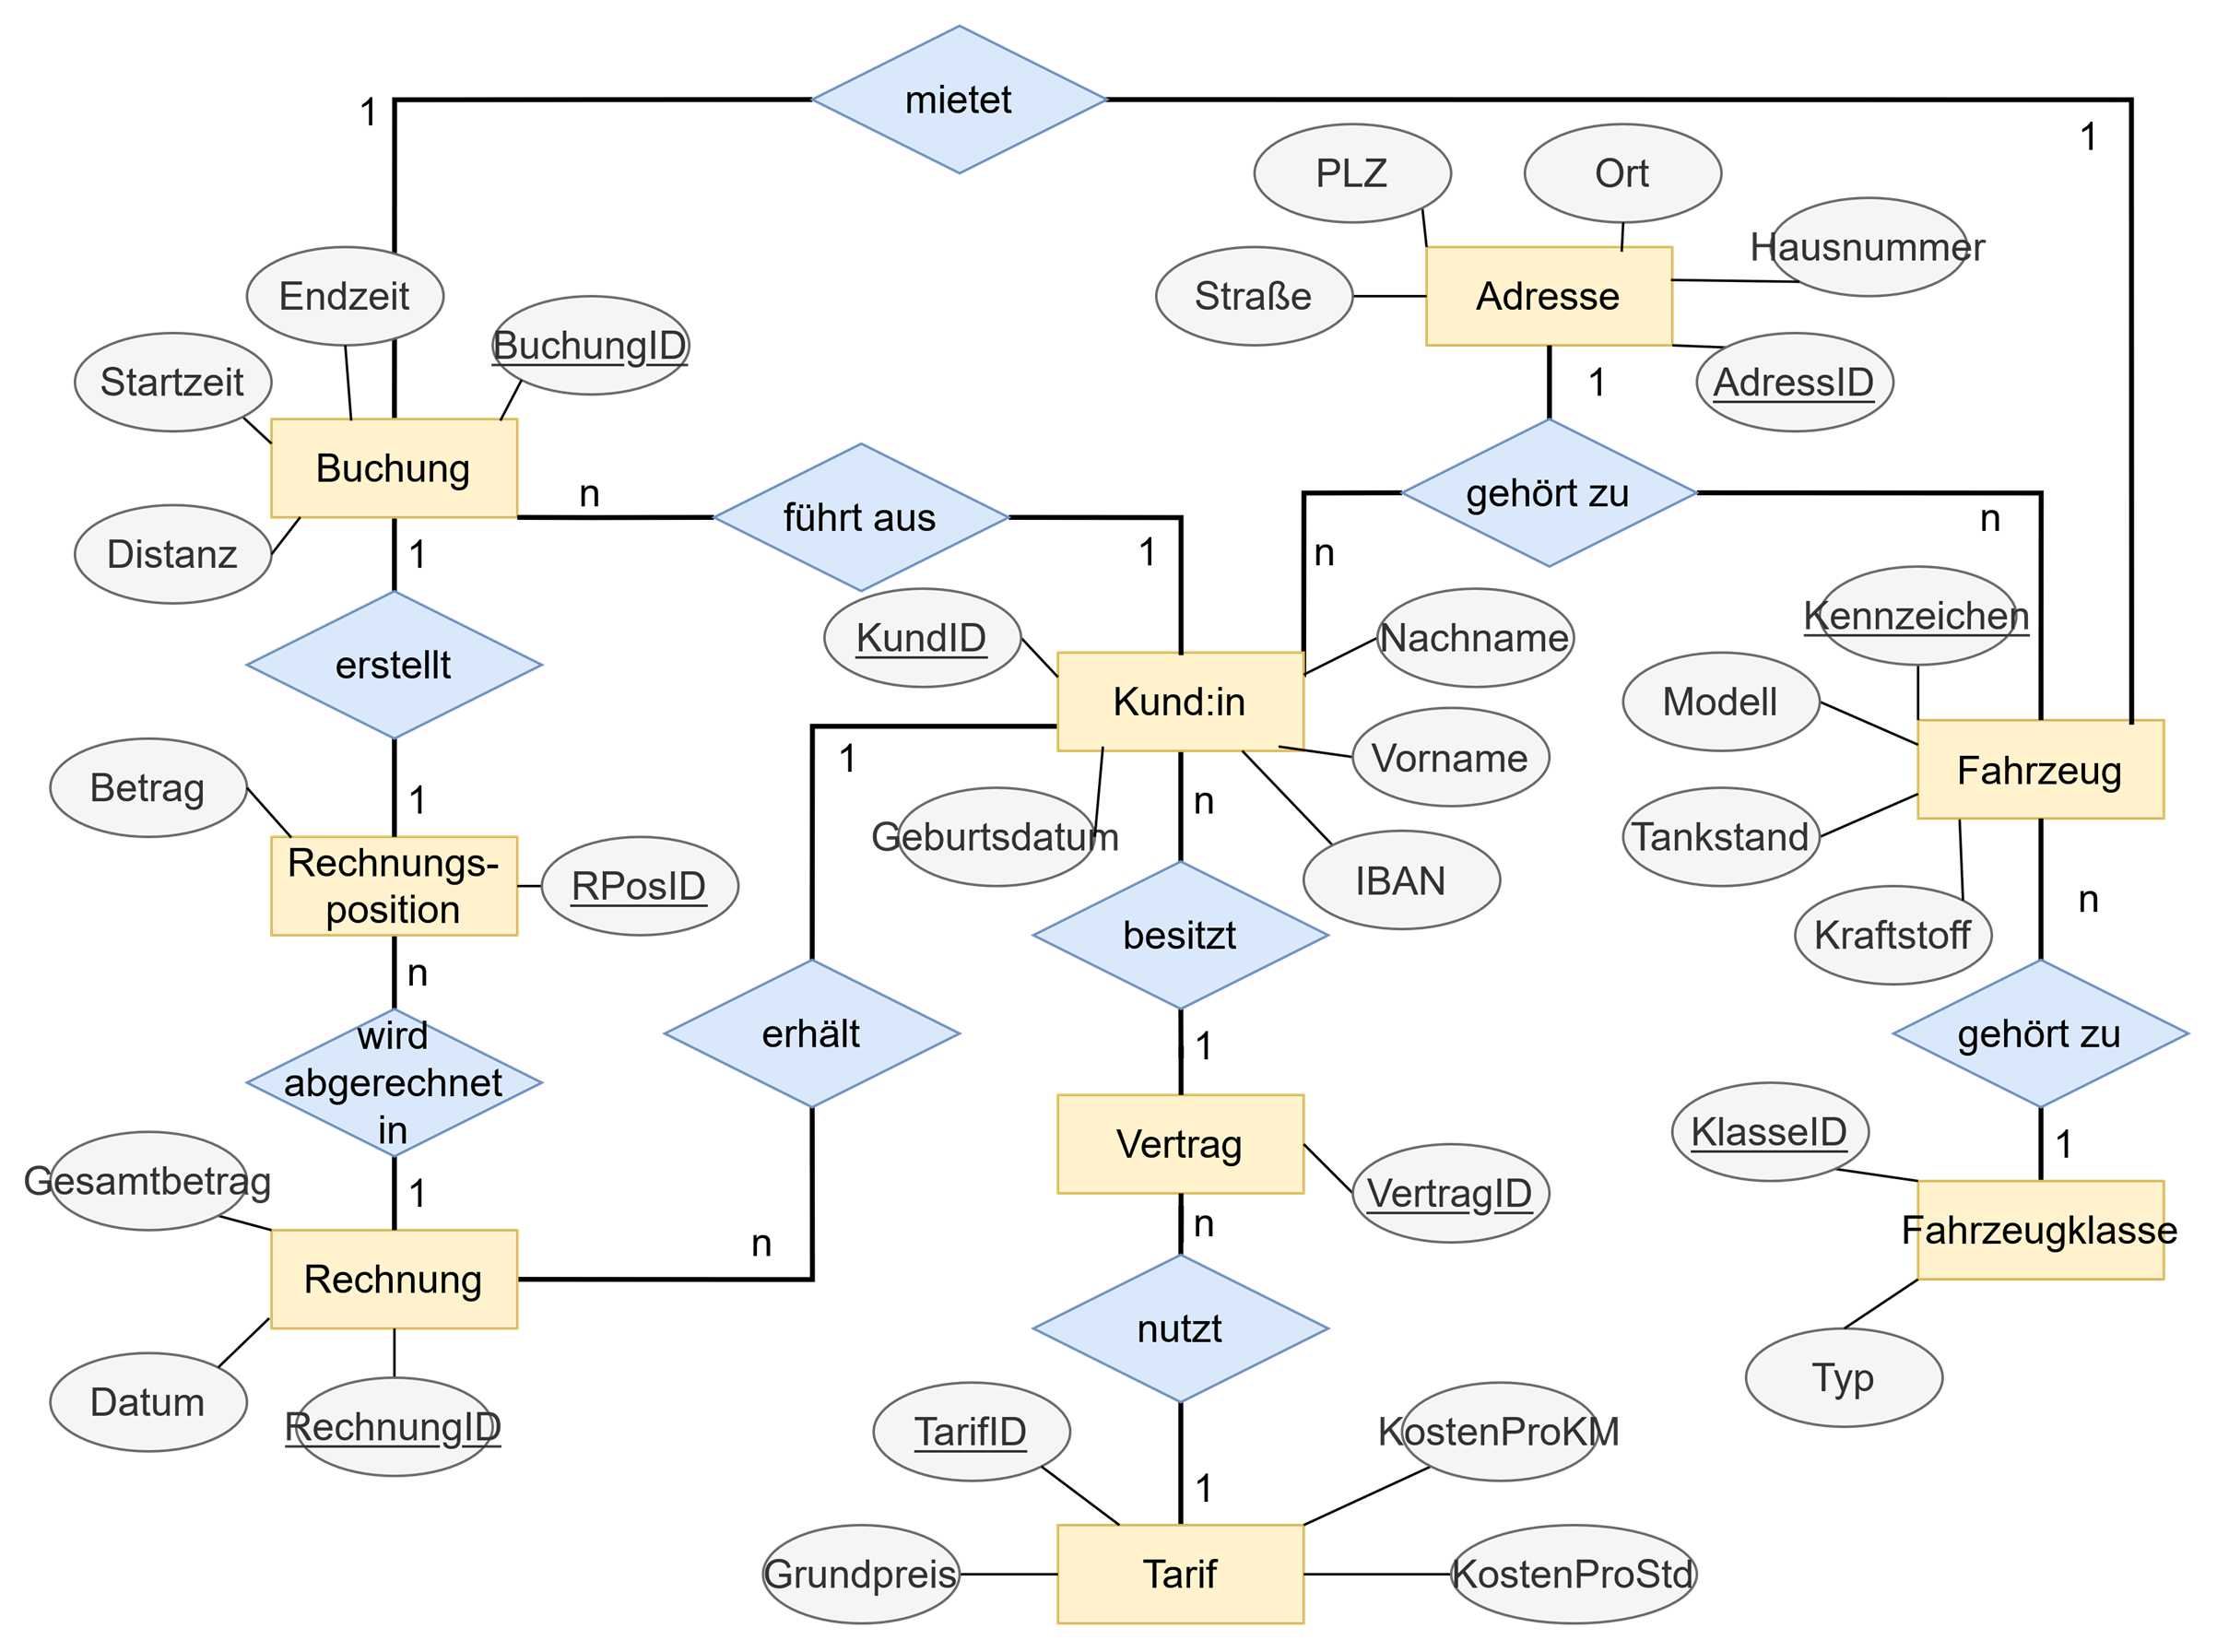
\includegraphics[width=\linewidth]{./pictures/ERM_Carsharing}
	\caption{ERM-Diagramm von der \glqq Carsharing Applikation\grqq.}
	\label{fig:ERM_Carsharing}
\end{figure}

In dem Entwurf des ER-Diagramms war insbesondere die Definition der Beziehungen eine gro\ss e Herausforderung. Die Beziehungen werden im nachfolgenden Relationenmodell in Fremdschlüssel übersetzt und sollten nur dort festgelegt werden, wo sie zwingend für die Definition der Entität notwendig sind. Beispielsweise wäre eine Buchung ohne die Festlegung eines Fahrzeugs nicht sinnhaft, weswegen in der Buchung eine Beziehung zu Fahrzeug definiert sein muss. In der späteren Umsetzung in eine reale Datenbank ist es sinnvoll programmatisch festzulegen, dass Datensätze ohne gültige Fremdschlüssel gar nicht erst angelegt werden dürfen. Dies stellt sicher, dass die Abfrage von Daten immer ein erwartetes Ergebnis liefert.

\paragraph{Schritt 2: Abbildung auf Relationenmodell}
Das ERM wird nun auf das Relationenmodell als spezifische Datenbankstruktur abgebildet. Für jeden Entitätstyp wurde in \ref{table:Buchung_main} bis \ref{table:Fahrzeugklasse_main} aus dem ER-Diagramm (\autoref{fig:ERM_Carsharing}) die entsprechende Tabelle erstellt. Hierbei wurden die Regeln der Normalisierung (siehe \autoref{subsec:Abbildung auf Relationenmodell}) bereits auf die Tabellen angewendet. Die einzelnen Datensätze (Entitäten) wurden in den Tabellen aus Gründen der Übersichtlichkeit nur durch Punkte angedeutet. Die Datensätze werden nachfolgend stattdessen im XML Format angegeben, das sich für die Darstellung besser eignet.

\begin{table}
	\centering
	\caption{Buchung}\label{table:Buchung_main}
	\begin{tabular}{l l l l l l} \toprule
		\underline{BuchungID} & Startzeit & Endzeit & Distanz & \textit{\underline{Kennzeichen}} & \textit{\underline{KundID} 	} \\ 
		\midrule
		\dots &  \dots & \dots  & \dots & \dots & \dots \\
		\bottomrule
	\end{tabular}
%\end{table}

%\begin{table}
	\centering
	\caption{Rechnung}\label{table:Rechnung_main}
	\begin{tabular}{l l l l l} \toprule
		\underline{RechnungID}  & Gesamtbetrag & Datum & \textit{\underline{KundID}} &  \textit{\underline{RPosID}}  \\ 
		\midrule
		\dots &  \dots & \dots  & \dots & \dots  \\
		\bottomrule
	\end{tabular}
%\end{table}

%\begin{table}
	\parbox{.49\linewidth}{
		\centering
		\caption{Rechnungsposition}\label{table:Rechnungsposition_main}
		\begin{tabular}{l l l} \toprule
			\underline{RPosID} & Betrag & \textit{\underline{BuchungID}} \\ 
			\midrule
			\dots &  \dots \\
			\bottomrule
		\end{tabular}
	}
	\parbox{.49\linewidth}{
		%\begin{table}
		\centering
		\caption{Adresse}\label{table:Adresse_main}
		\begin{tabular}{l l l l l} \toprule
			\underline{AdressID} & Stra\ss e & Nr & PLZ & Ort \\ 
			\midrule
			\dots &  \dots & \dots  & \dots & \dots \\
			\bottomrule
		\end{tabular}
		%\end{table}
	}
%\end{table}

%\begin{table}
	\centering
	\caption{Kund:in}\label{table:Kund_main}
	\begin{tabular}{l l l l l l} \toprule
	\underline{KundID} 	& Vorname & Nachname & Geburtsdatum & IBAN & \textit{\underline{AdressID}} \\ 
	\midrule
	\dots &  \dots & \dots  & \dots & \dots & \dots \\
	\bottomrule
	\end{tabular}
%\end{table}

%\begin{table}
	\centering
	\caption{Tarif}\label{table:Tarif_main}
	\begin{tabular}{l l l l} \toprule
		\underline{TarifID} & Grundpreis & KostenProKM & KostenProStd \\ 
		\midrule
		\dots &  \dots & \dots  & \dots  \\
		\bottomrule
	\end{tabular}
%\end{table}

%\begin{table}
	\parbox{.45\linewidth}{
		\centering
		\caption{Vertrag}\label{table:Vertrag_main}
		\begin{tabular}{l l l l} \toprule
		\underline{VertragID} &  \textit{\underline{KundID}} & \textit{\underline{TarifID}} \\ 
		\midrule
		\dots &  \dots & \dots  \\
		\bottomrule
		\end{tabular}
	}
	\parbox{.45\linewidth}{
		\centering
		\caption{Fahrzeugklasse}\label{table:Fahrzeugklasse_main}
		\begin{tabular}{l l} \toprule
			\underline{KlasseID} & Typ\\ 
			\midrule
			\dots &  \dots \\
			\bottomrule
		\end{tabular}
	}
%\end{table}

%\begin{table}
	\centering
	\caption{Fahrzeug}\label{table:Fahrzeug_main}
	\begin{tabular}{l l l l l l} \toprule
		\underline{Kennzeichen} & Modell & Tankstand & Kraftstoff &  \textit{\underline{KlasseID}} & \textit{\underline{AdressID}} \\ 
		\midrule
		\dots &  \dots & \dots  & \dots &  \dots & \dots  \\
		\bottomrule
	\end{tabular}
\end{table}

Die folgende XML codierte Darstellung zeigt einen Datensatz aus der Tabelle \textit{Rechnung}. Das XML Format erlaubt eine hierarchische Darstellung von Datensätzen. Dadurch können Sichtweisen, aus denen heraus die Datensätze betrachtet werden übersichtlich dargestellt werden. Die gewählte Sichtweise, aus der ein Datensatz in XML dargestellt wird, bestimmt die logische bzw. hierarchische Struktur der verknüpften Entitäten. Für den XML-Codeausschnitt wurde die Sichtweise der Beispiel-Rechnung \glqq R1B3C\grqq) gewählt, sodass Kunde \glqq K100A\grqq\ und Rechnungspositionen \glqq P2341G\grqq, \glqq PAB234\grqq als untergeordnete Fremdschlüssel-Attribute auftauchen. Wie im ERM-Diagramm in \autoref{fig:ERM_Carsharing} dargestellt sind diese durch Fremdschlüssel verknüpften Informationen wichtig für den Vorgang der Rechnungserstellung. Analog würden sich für die anderen Entitäten sehr unterschiedliche Sichtweisen und somit Darstellungen der primären Attribute, sowie sekundärer über Fremdschlüssel verknüpfter Attribute ergeben. Eine flache Darstellung von Datensätzen im XML Format ohne Hierarchien ist im Anhang (\autoref{subsec:XMLcode}) dargestellt und bildet alle Datensätze ab für das beispielhaft erstellte DMBS erstellt wurden.

\begin{lstlisting}[language=XML]
<?xml version="1.0" encoding="UTF-8"?>
<CarsharingDatensaetze>
    <!--Beispieldatensatz Rechnung?-->
    <RechnungID id="R1B3C">
        <Gesamtbetrag>123.34</Gesamtbetrag>
        <Datum>Schmidt</Datum>
        <KundID id="K100A">
            <Vorname>Ralf</Vorname>
            <Nachname>Hanser</Nachname>
            <Geburtsdatum>13.04.1999</Geburtsdatum>
            <IBAN>DE89370400440532013000</IBAN>
            <VertragID id="V2361C">
                <...>
            </VertragID>
            <AdressID id="A2361C">
                <...>
            </AdressID>
        </KundID>
        <RPosID id="P2341G">
            <Betrag>33.50</Betrag>
            <BuchungID id="B34DG">
        </RPosID>
        <RPosID id="PAB234">
            <Betrag>89.84</Betrag>
            <BuchungID id="C3123">
        </RPosID>
    </RechnungID>
</CarsharingDatensaetze>
\end{lstlisting}


\subsection{Datensätze in SQLite und Racket}
%Definieren Sie die Klassen auch als Code in Racket oder in einer anderen objektorientierten Programmiersprache. Die Beziehungen zwischen den Klassen müssen Sie nicht darstellen, dürfen Sie aber.
Die theoretischen Betrachtungen werden in diesem Abschnitt in ein relationales DBMS übertragen. Für die Realisierung wird die Programmiersprache Racket zusammen mit dem in Racket bereits implementierten DBMS SQLite verwendet. Der komplette Programm-Code (in Racket) um das DBMS in der entworfenen Form umzusetzen ist im Anhang in \autoref{subsec:SQLcode} gegeben. Beispielhaft wird dort auch ein Datensatz komplett angelegt und Beispielabfragen in SQL ausgeführt.

Zunächst wird eine SQlite Datenbank-Datei (.db) namens \glqq carsharing.db\grqq\ erstellt. Der Befehl \ir{PRAGMA foreign\_keys = ON} stellt sicher, dass Fremdschlüssel-Attribute erst definiert werden können wenn der Datensatz auf den sie verweisen existiert.
\begin{lstlisting}[language=racketSQL]
#lang racket
;; Carsharing Example: Connecting to SQLite ;; 
(require db)
;; Connect to (or create) a database file named "carsharing.db" ;;
(define conn
    (sqlite3-connect #:database "carsharing.db"
                     #:mode 'create))
;; Enable foreign key enforcement ;;
(query-exec conn "PRAGMA foreign_keys = ON;")
\end{lstlisting}

Über das \glqq conn\grqq\ Objekt kann die Datenbank beschrieben werden. Zunächst müssen die Entitätstypen über den Befehl \ir{CREATE TABLE} definiert werden. Die Definition der Attribute erfolgt zeilenweise über die Definition von Attributsname Datentyp und weiteren Typ-Eigenschaften. Das Schlüsselwort \ir{PRIMARY KEY} markiert den Primärschlüssel. Fremdschlüssel werden über die \ir{FOREIGN KEY} Definition in einer weiteren Zeile mit ihrer Referenz auf die Fremd-Tabelle definiert. Zusätzlich findet sich in der letzten Zeile das Schlüsselwort \ir{UNIQUE(..)}, welches festlegt, dass neben dem Primärschlüssel auch die Kombination aus den hier definierten Feldern nicht dupliziert vorliegen darf. Dadurch werden Duplikatseinträge verhindert, die durch den Befehl \ir{AUTOINCREMENT} im Primärschlüssel durch wiederholtes Anlegen von gleichen Einträgen entstehen können.
\begin{lstlisting}[language=racketSQL]
;; Create <Buchung> table ;; 
(query-exec conn
	"CREATE TABLE IF NOT EXISTS Buchung (
		id INTEGER PRIMARY KEY AUTOINCREMENT,
		startzeit TEXT NOT NULL,
		endzeit TEXT NOT NULL,
		distanz REAL,
		FahrzeugID TEXT NOT NULL,
		KundID INTEGER NOT NULL,
		FOREIGN KEY(FahrzeugID) REFERENCES Fahrzeug(Kennzeichen),
		FOREIGN KEY(KundID) REFERENCES Kunde(KundID),
		UNIQUE(startzeit, FahrzeugID, KundID)
		);")
\end{lstlisting}

Die Tabelle wird nun mit den Schlüsselwörtern \ir{INSERT ... INTO} mit Datensätzen gefüllt. \ir{IGNORE} oder \ir{REPLACE} verhindern das Erstellen von Duplikaten. Racket erlaubt das Verwenden von Platzhalter Argumenten \glqq ?\grqq\, welche in dem folgenden Beispiel verwendet wurden und die Übersichtlichkeit verbessern\footnote{Weitere Gründe für Platzhalter Argumente finden sich in der Racket Dokumentation: https://docs.racket-lang.org/sql/index.html, Zugriff am 28.11.2025}.
\begin{lstlisting}[language=racketSQL]
;; "Insert entry in <Buchung> table" ;;
(query-exec conn
	"INSERT OR IGNORE INTO Buchung (startzeit, endzeit, distanz, FahrzeugID, KundID)
	VALUES (?, ?, ?, ?, ?)"
	"2025-05-29 14:16:00" "2025-11-30 18:16:00" 15.30 "RO-CJ-262" 1)
\end{lstlisting}

Beispielhaft sollen nun Abfragen der Datenbank gezeigt werden. Abfragen werden in Racket über die \glqq conn\grqq\ Schnittstelle mittels der SQLite Syntax erstellt. Um die Abfrageergebnisse nachvollziehen zu können sind die Datensätze, welche in der Carsharing Datenbank eingetragen wurden in \autoref{subsec:XMLcode} als XML Struktur dargestellt. Im nachfolgenden Programmcode sind zwei Abfragen des Typs: \ir{SELECT ... FROM ... INNER JOIN ... ON ...} gegeben, welche sich dafür eignen um die Spalten zweier Tabellen auf Basis einer Identität (hier Identität von Primärschlüsseln und Fremdschlüsseln) abzufragen. Die erste Abfrage verwendet die Tabelle Kunde und Buchung um herauszufinden welche Buchungen von welchen Kund:innen durchgeführt wurden. Die zweite Abfrage liefert alle Fahrzeuge mit ihren zugehörigen Standortadressen, so dass Kund:innen-Adressen nicht mit aufgeführt werden.
\begin{lstlisting}[language=racketSQL]
;; "Query bookings from all customers" ;;
(define Buchungseintraege
	(query-rows conn
		"SELECT Vorname, Nachname, IBAN, FahrzeugKennzeichen, distanz
		FROM Kunde
		INNER JOIN Buchung on Buchung.KundID = Kunde.KundID"))
(for ([r Buchungseintraege])
	(printf "~a\n" r))
;; "Query parking locations of cars only (w/o customer adresses)" ;;
(define FahrzeugAdressen
	(query-rows conn
		"SELECT Modell, Kennzeichen, Strasse, Nr, PLZ, Ort
		FROM Adresse
		INNER JOIN Fahrzeug on Fahrzeug.AdressID = Adresse.AdressID;"))
(for ([r FahrzeugAdressen])
	(printf "~a\n" r))
\end{lstlisting}

Über die \ir{printf} Funktion werden die Variablen (Racket-Typ Liste), welche die Ergebnisse der Abfragen speichern ausgegeben. Für die erste Abfrage der Buchungseinträge erhält man:
\begin{lstlisting}[language=racketSQL]
#(Thomas Gerrer DE89370400440532013000 RO-CJ-262 15.3)
\end{lstlisting}
Und für die zweite Abfrage:
\begin{lstlisting}[language=racketSQL]
#(Fiat Punto RO-CJ-262 Eisenhutstr. 60 72072 Tuebingen)
\end{lstlisting}

Die hier gezeigte Umsetzung der Carsharing App \glqq TeilAuto Neckaralb\grqq in SQLite und Racket zeigt nur eine oberflächliche Betrachtung, welche einen Einstieg in die Welt relationaler Datenbanksystemen geben soll. Viele Aspekte eines realen DBMS für eine solche Anwendung wurden hier nicht berücksichtigt. Im Abschluss dieser Arbeit werden die Ergebnisse dieser Arbeit zusammengefasst und die Aspekte diskutiert, die in einer realen Datenbank zusätzlich berücksichtigt werden sollten.






























